\documentclass{standalone}
\usepackage{tikz}
\usepackage{tikzpeople}
\usepackage{cryptocode}
\begin{document}
			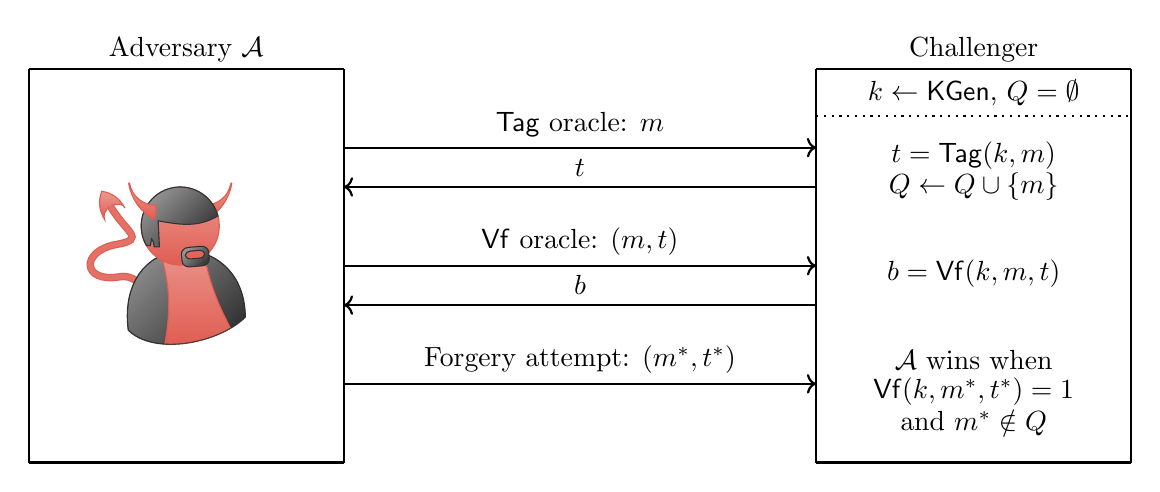
\begin{tikzpicture}
				
				\node[] (lblAdv) at (2,3.25) {Adversary $\mathcal{A}$};
				\draw[-,thick] (0,-2)--(4,-2);
				\draw[-,thick] (4,-2)--(4,3);
				\draw[-,thick] (4,3)--(0,3);
				\draw[-,thick] (0,3)--(0,-2);
				
				\node[devil, evil, minimum size=1.5cm] (Attacker) at (2,.5) {};
				
				\node[] (lblCha) at (12,3.25) {Challenger};
				\draw[-,thick] (10,-2)--(14,-2);
				\draw[-,thick] (14,-2)--(14,3);
				\draw[-,thick] (14,3)--(10,3);
				\draw[-,thick] (10,3)--(10,-2);
				
				\node[] (KeyGen) at (12,2.7) {$k \gets \mathsf{KGen}$, $Q = \emptyset$};
				\draw[-, thick, dotted] (10,2.4) -- (14,2.4);
				
				\draw[->, thick] (4,2) -- (10,2) node[midway, above] {\textsf{Tag} oracle: $m$};
				\node[] (Enc) at (12,1.9) {$t = \mathsf{Tag}(k,m)$};
				\node[] (Add) at (12,1.5) {$Q \gets Q \cup \{m\}$};
				\draw[<-,thick] (4,1.5) -- (10,1.5) node[midway, above] {$t$};

				\draw[->,thick] (4,0.5) -- (10,0.5) node[midway,above] {\textsf{Vf} oracle: $(m,t)$};
				\draw[<-,thick] (4,0) -- (10,0) node[midway,above] {$b$};
				\node[] (Vf) at (12,0.4) {$b = \mathsf{Vf}(k,m,t)$};
				
				\draw[->, thick] (4,-1) -- (10,-1) node[midway, above] {Forgery attempt: $(m^*, t^*)$};
				\node[] (WinVfy) at (12,-.7) {$\mathcal{A}$ wins when};
				\node[] (WinVfy) at (12,-1.1) {$\mathsf{Vf}(k, m^*,t^*) = 1$};
				\node[] (WinVfy) at (12,-1.5) {and $m^* \notin Q$};
				
			\end{tikzpicture}
\end{document}
